\documentclass[a4paper,10pt]{article}

\usepackage[english]{babel}
\usepackage{graphicx}
\usepackage[colorlinks, allcolors=black]{hyperref}
\usepackage{geometry}
\geometry{tmargin=3cm, bmargin=3cm, lmargin=2.4cm, rmargin=2.2cm}
\usepackage{todonotes} %Used for the figure placeholders
\usepackage{ifthen}
\usepackage{parskip}
\usepackage{hyperref}
\usepackage{caption}
\usepackage{listings}
\usepackage{tabu}
\usepackage{rotating}
\usepackage{multirow}
\usepackage{pmboxdraw}
\usepackage{setspace}
\usepackage{subcaption}
\usepackage{alltt}
\usepackage{amsmath}

\graphicspath{{./images/}}

\begin{document}
\newboolean{anonymize}
% Uncomment to create an anonymized version of your report
%\setboolean{anonymize}{true}

\begin{titlepage}
    \newpage
    \thispagestyle{empty}
    \frenchspacing
    \hspace{-0.2cm}
    
\includegraphics[height=3.4cm]{sedes}
    \hspace{0.2cm}
    \rule{0.5pt}{3.4cm}
    \hspace{0.2cm}
    \begin{minipage}[b]{8cm}
        \Large{KULeuven}\smallskip\newline
        \large{}\smallskip\newline
        \textbf{Department of\newline Computer Science}\smallskip
    \end{minipage}
    \hspace{\stretch{1}}
    \vspace*{3.2cm}\vfill
    \begin{center}
        \begin{minipage}[t]{\textwidth}
            \begin{center}
                \LARGE{\rm{\textbf{\uppercase{Computer Vision (H02A5a)}}}}\\
                \Large{\rm{Project: Dental Radiographs}}
            \end{center}
        \end{minipage}
    \end{center}
    \vfill
    \hfill\makebox[8.5cm][l]{%
        \vbox to 7cm{\vfill\noindent
            \ifthenelse{\boolean{anonymize}}{%
                {\rm \textbf{Anonymized}}\\
                {\rm Academic year 2015--2016}
            }{%
                {\rm \textbf{Jorik De Waen (r0303087)}}\\ [2mm]
                {\rm Academic year 2015--2016}
            }
        }
    }
\end{titlepage}


\newpage
\section{Introduction}
The assignment for this report is to extract the 4 top and bottom incisors from panoramic dental radiographs using a limited set of training data. This provides an interesting challenge as several distinct steps need to come together to form a working algorithm. The algorithm I ended up developing works entirely without human input and works reasonably well with some clear weaknesses.

\section{Active Shape Models}
The first step in the solution is building the Active Shape Model for each of the eight teeth. 14 radiographs have been provided with 40 landmarks for each of the eight teeth. Since the solution works on a per-tooth level, the landmarks are grouped by teeth instead of by radiograph. Before a model can be constructed from these landmarks, they need to be normalized first. Each set of 40 landmarks is translated to place the mean of the landmarks on the origin. After that, the landmarks in each set are scaled such that the average distance from the origin is one. As the final step, each set of landmarks is rotated to match the orientation of the first set of landmarks for that specific tooth.
\\
Once all landmarks have been normalized, Principal Component Analysis is used to construct a basis for feature space of each of the 8 teeth. Note that the mirrored dataset is also used for the PCA. Once this basis has been calculated, each set of landmarks is projected onto the space spanned by the basis to collect statistical data. For each dimension in the feature space, the standard deviation of the values of each dataset for that dimension will later determine what will be considered an acceptable shape for a tooth.

\begin{figure}[h]

\begin{tabular}{cc}
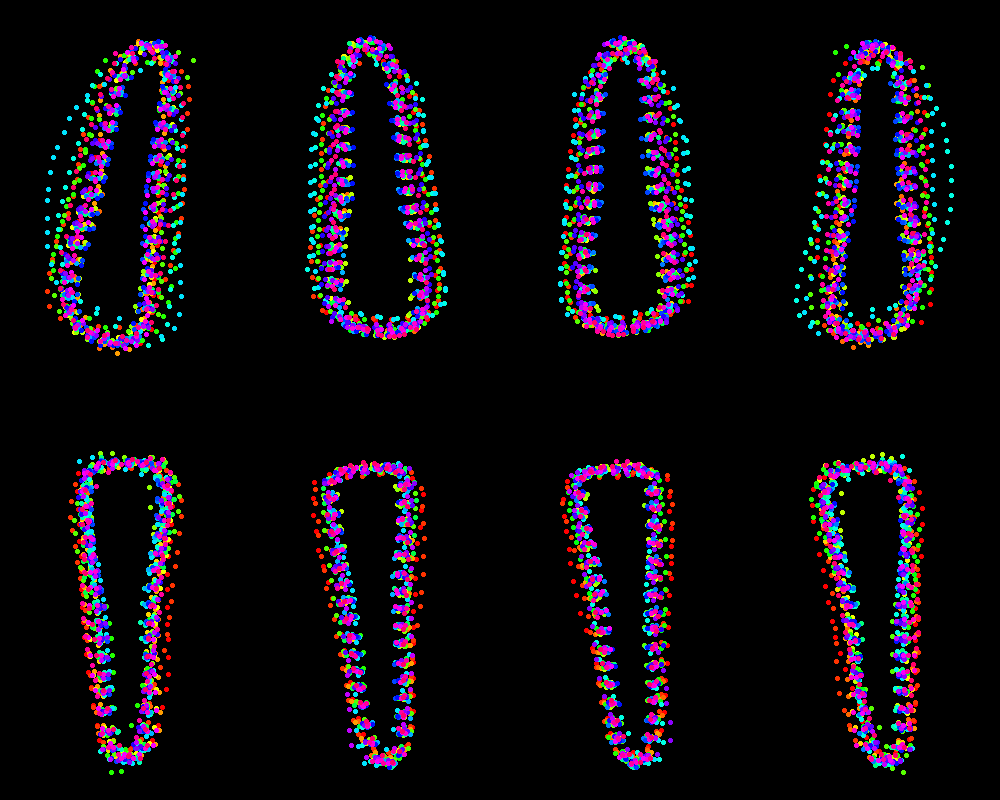
\includegraphics[width=80mm]{landmarks.png} & 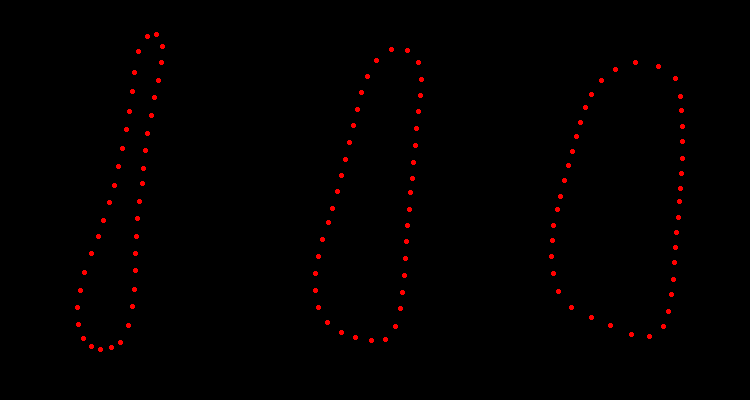
\includegraphics[width=80mm]{modelvar-0-0.png}\\
 
\end{tabular}
 \caption{The left image displays all normalized sets of landmarks grouped by tooth, overlaid on eachother. The right image displays the effect of modifying the first (most important) coordinate by 3 standard deviations down (on the left) or up (on the right). The middle tooth is the average tooth.}
\end{figure}

\newpage
\section{Radiograph Processing}
The provided radiographs are complex images with significant amounts of noise and a relatively low contrast. Several steps of processing are needed to extract usable information from these images. \\

An easy first step to bring out the information the algorithm needs is to crop as much as possible. This drastically recudes the computational workload and focuses the image on the part we're interested in. By doing this, 85\% of the image can be ignored without removing any relevant information.
\\
The next observation when looking at the images is the large variation in lighting between the radiographs as well as between different spots in the same radiograph. To counteract that, the cropped image is passed through a homomorphic filter. This is a high-pass filter that removes a large part of the variation in lighting.
\\\\
Two different operations are applied on the homomorphically filtered image. The first operation is is normalizing the histogram of the image. This operation calculates the histogram of the image and remaps every distinct intensity level to another level in a way that spreads them out evenly. This maximizes the contrast between the lowest and highest intensities found in the image. This is specifically useful because it will map the inside of the mouth to very low values. This will be used to detect where the mouth is.\\\\
The second operation that is applied on the homomorphically filtered image is a Sobel filter. This is an edge detection filter. The higher the difference in intensity between one pixel and it neighbors, the higher the intensity in the filtered image. Sobel filters look for gradients in the x and y  separately, these gradients are combined by taking the root of the sum of their squares. However, this intensity of the gradient is not the only information which can be obtained from this. The x and y values of the gradient are a vector together. This vector depicts the direction of the slope. This direction is very useful in other parts of the algorithm. \\
However, the result of the Sobel filter is very noisy. This is because the input image itself is noisy to begin with, and the homomorphic filter also tends to exaggerate noise because it is a high-pass filter. To counteract this, the intensities from the Sobel filter and the directions of the gradients are stored seperately. The intensities are passed through a very aggressive denoise filter and the directions of the gradients are normalized.

\begin{figure}[h]
\centering
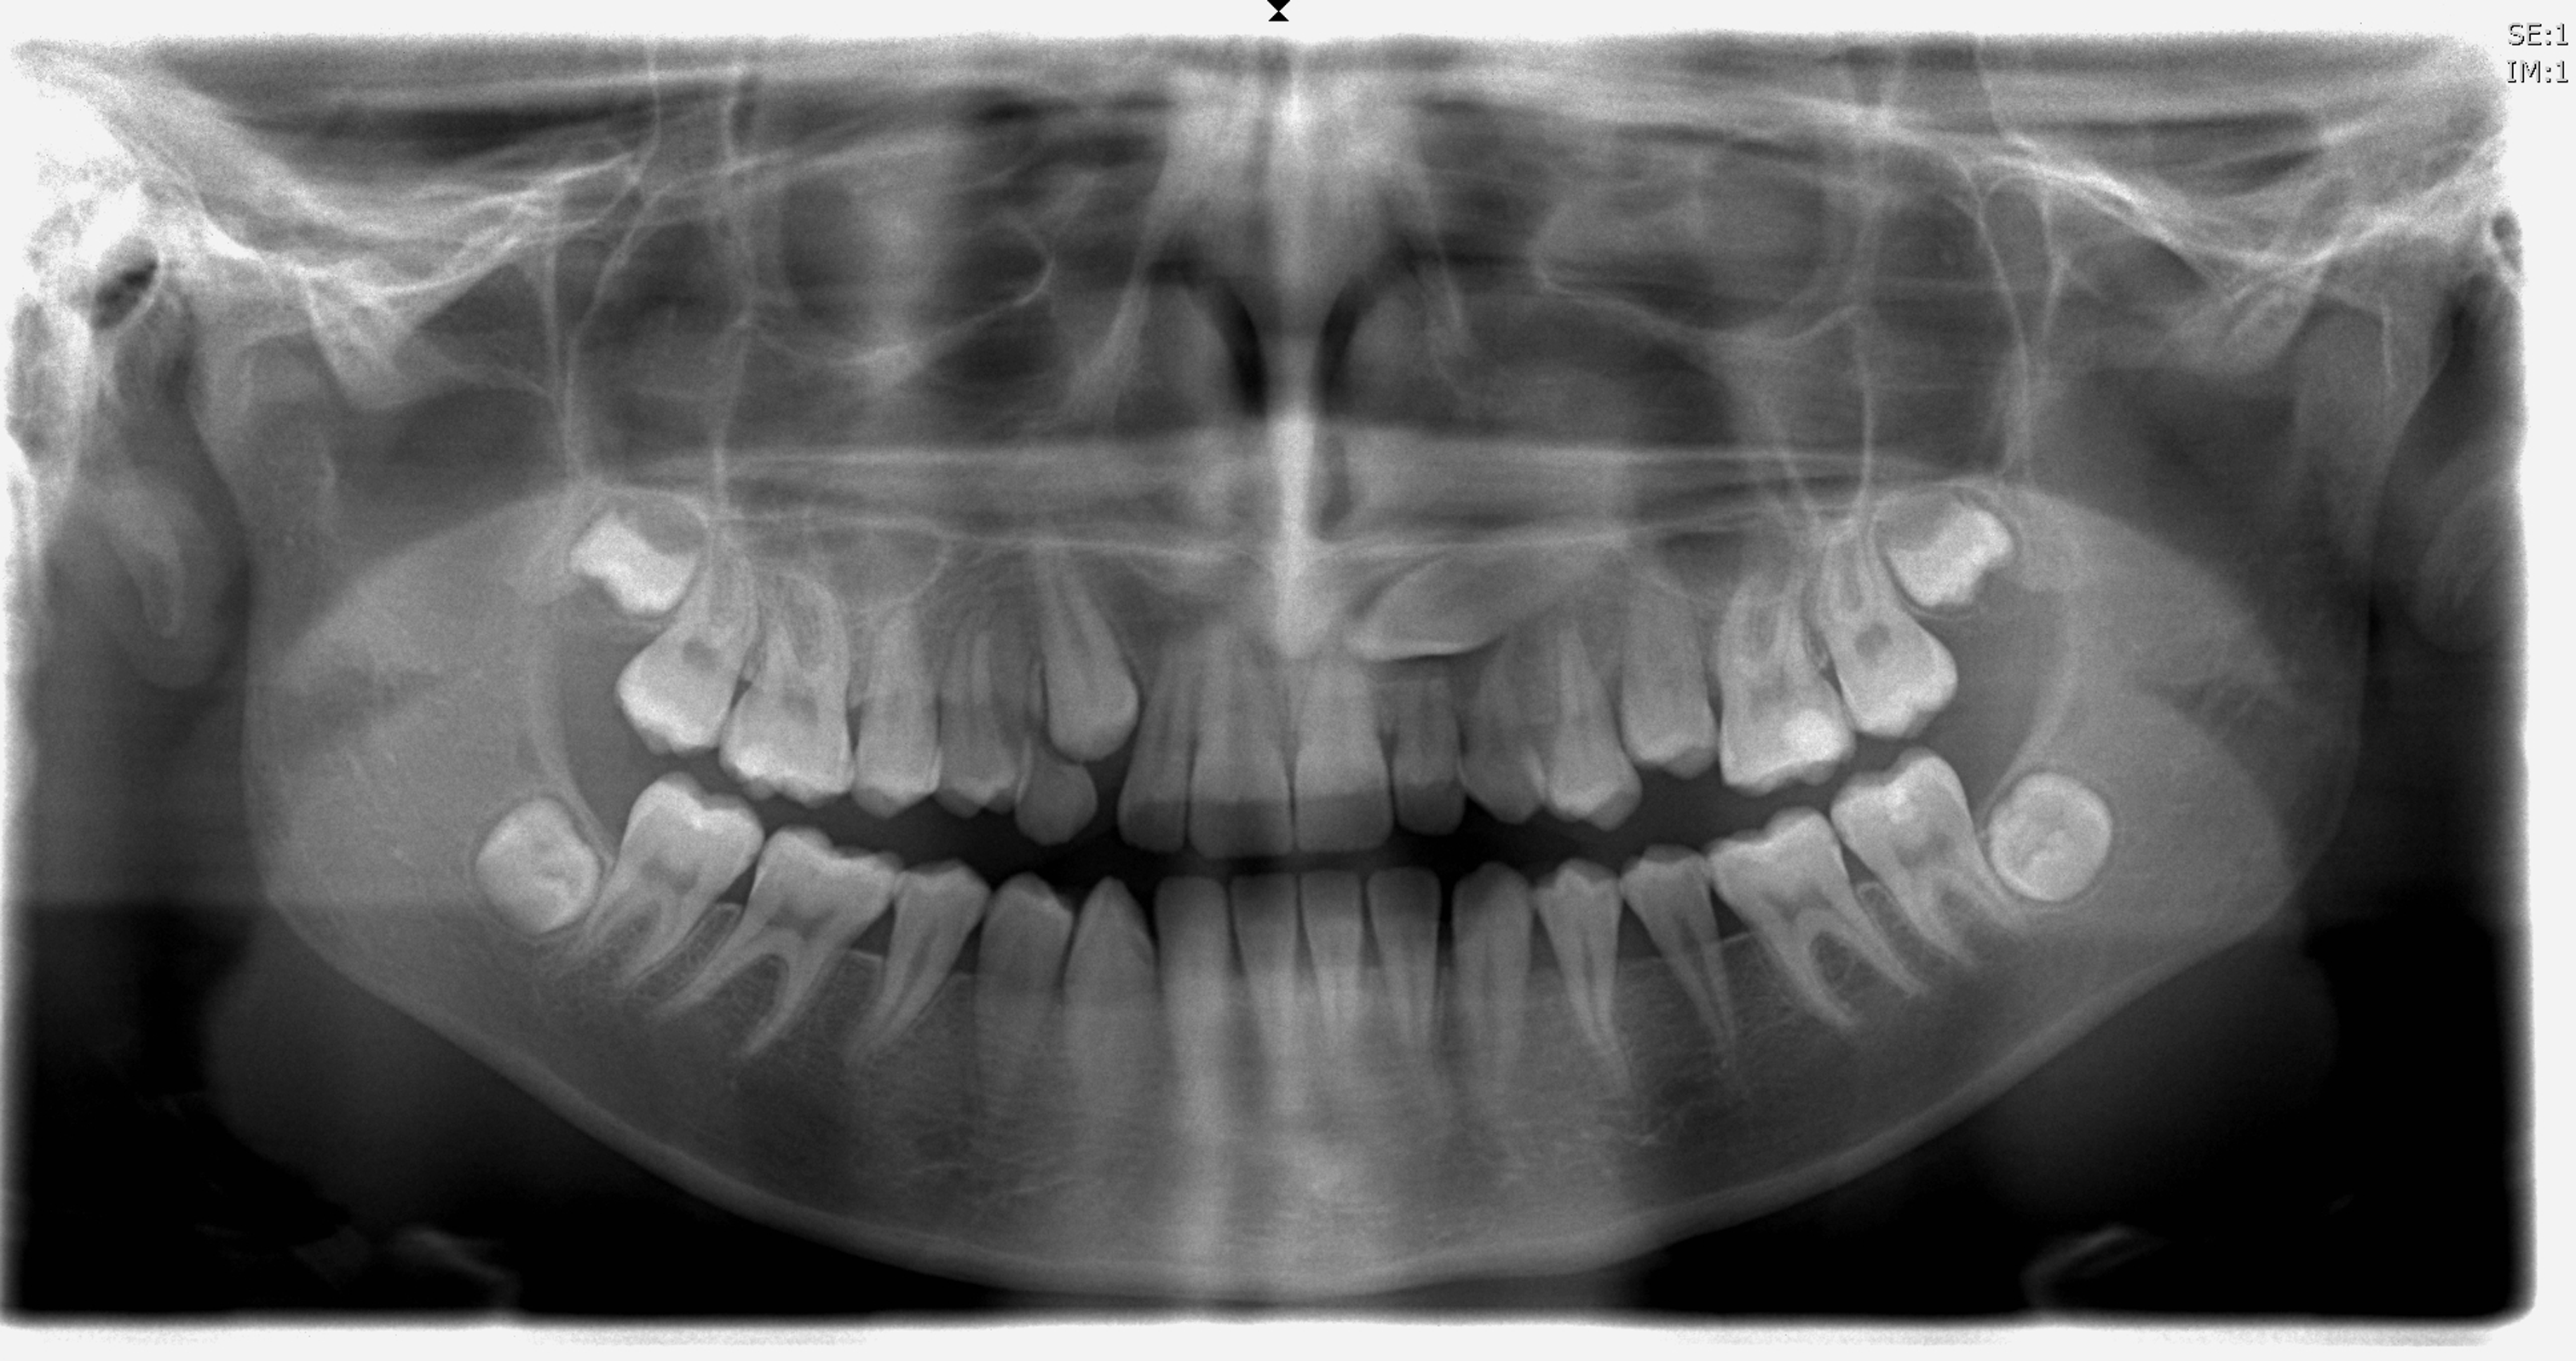
\includegraphics[width=160mm]{raw.png}
 \caption{An example of a raw input radiograph.}
\end{figure}


\begin{figure}[!h]

\begin{tabular}{cccc}
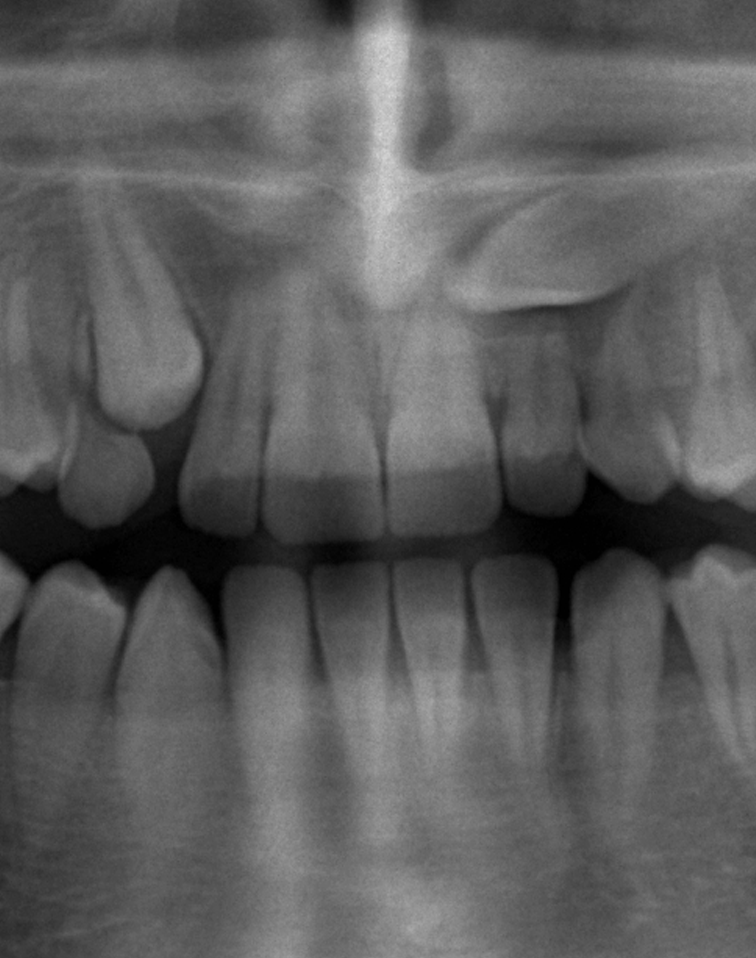
\includegraphics[width=80mm]{cropped.png} & 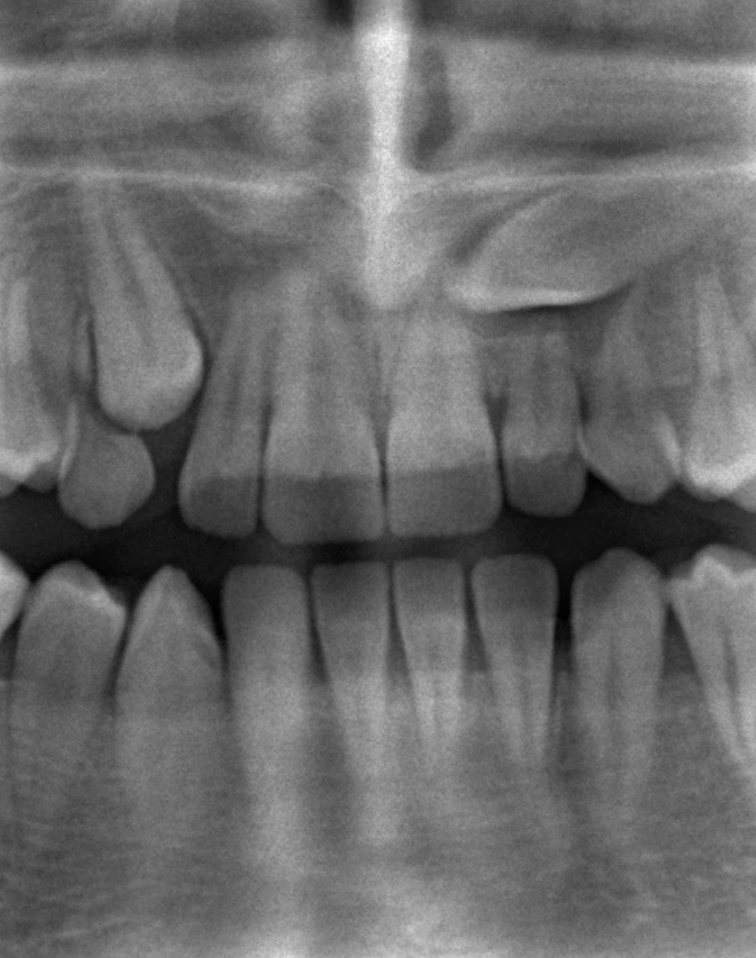
\includegraphics[width=80mm]{homo.png} \\
 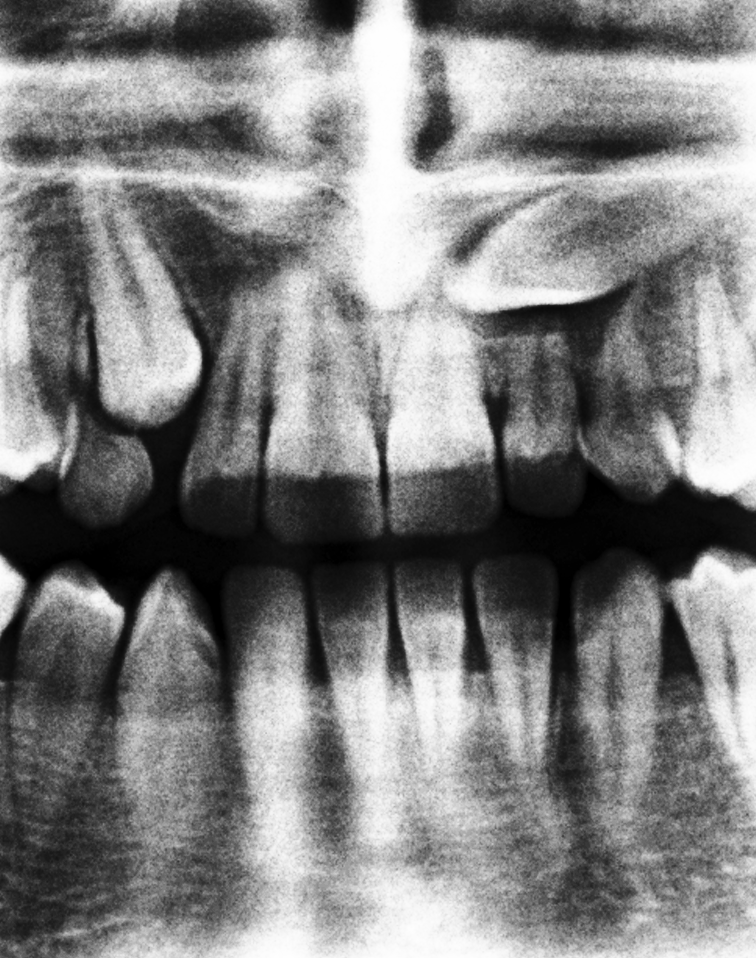
\includegraphics[width=80mm]{norm.png} & 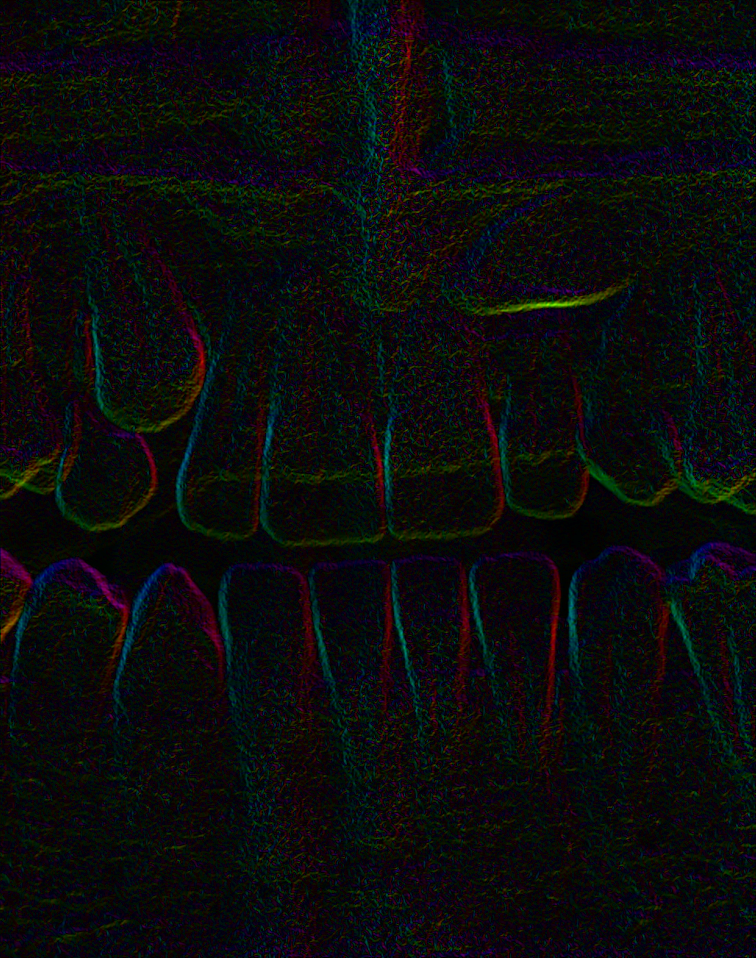
\includegraphics[width=80mm]{gradients.png} \\
 
\end{tabular}
 \caption{The different steps of the processing of the radiographs. The top left corner image is the cropped image. The image in the top-right corner shows the result after homomorphic filtering. The image in the bottom left corner shows the result after histogram normalization. The image in the bottom right corner is the result of the Sobel filter after the noise removal step. The directions of the Sobel vectors are encoded as the hue of the color, while the brightness of the color depicts the intensity. }
\end{figure}


\section{Determining starting positions}
The last step that needs to be done before the fitting algorithm can work is to find starting positions. Because the teeth have a large variation in position, rotation and size I have decided to let the algorithm start at the edge between the teeth and the ``hole'' of the mouth. That is the bottom edge of the tooth for the toop teeth and the top edge of the tooth for the bottom teeth.
\\\\
My first attempt at this simply used the mean locations of these points from the dataset. The problem with this approach is that the standard deviation of the x coordinate is anywhere between 15 and 30 pixels and the standard deviation of the y coordinate is around 50 pixels. This is too much for a local search algorithm to handle. The second idea was to try to use an Active Appearance Model. However I could not find a suitable model for panoramic radiographs and constructing one myself would be extremely difficult.
\\\\
Eventually, I settled on manually programming an algorithm that would detect the eight starting points needed for the fitting algorithm. It consists of several different steps. At each step, the algorithm extracts more information about the position of the teeth based on the previous step.

\subsection{Position of the mouth}
The first step is determining the vertical position of the mouth. The image with the normalized histogram as described above is used for this. The mouth should have very low intensity values, so the image is inversly thresholded at around 20\% intensity. This will make all dark sections of the image white and the rest black. Because the image is cropped, the mouth covers the full width of the image. By averaging the values for each row and picking the row with the maximum value, the vertical position of the mouth is found.

\begin{figure}[h]
\centering
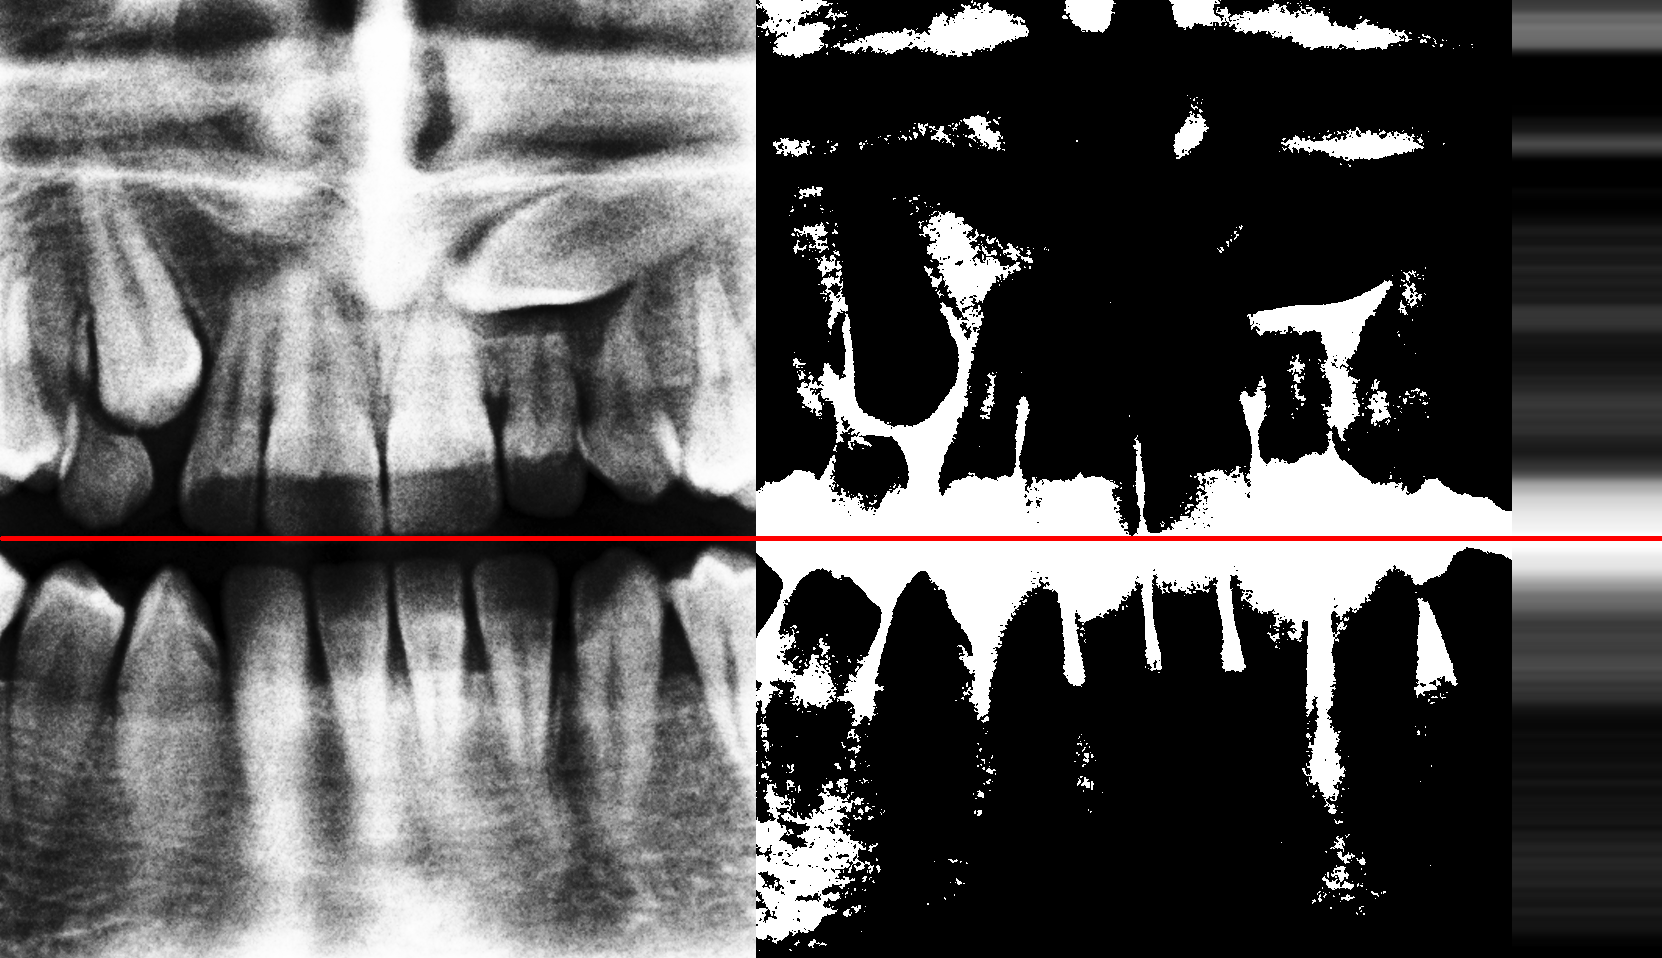
\includegraphics[height=50mm]{mouth_vis.png}
 \caption{Rough detection of the vertical position of the mouth. The left image shows the normalized image, the right image shows the result of thresholding values to everything that's below 20\% intensity. The bar on the right shows the average intensity for each row in the thresholded image. The red line indicates for which row this average is the highest}
\end{figure}

\subsection{Rough Y coordinates of the top and bottom groups of teeth} 
The next step is determining roughly where the upper and lower teeth are located. In some radiographs, the upper and lower teeth are just a few pixels apart while in others there is a significant gap. To counteract the possibility of a gap the next step will work relative to the edges of the upper and lower teeth separately. The y coordinate for the center of the mouth from the previous step is a rough approximation and may be slightly above or below the actual position. To counteract that, we need to look on both sides of that y coordinate. For instance: For the bottom teeth the algorithms starts slightly above the mouth's y coordinate and stop a good distance below it. The problem here is that the algorithm needs to distinguish between the edge of the upper teeth and the lower teeth. This is where the Sobel gradient vectors come in. For the bottom teeth, we know that we are looking for an edge that goes from dark to bright when going downwards. By using the scalar product between the desired gradient vector and the actual vector, the algorithm can easily filter out the wrong edge. After that, the rows from the result of the scalar product can be averaged again and the first average that reaches a certain threshold is selected as the starting position for that set of teeth. Only a narrow segment is used for this because the different teeth can be at an angle and have very different positions. By limiting this to a narrow segment in the middle we get a good approximation for the middle teeth.
\begin{figure}[h]
\centering
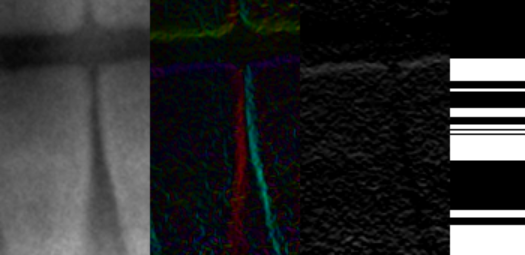
\includegraphics[height=50mm]{teeth_vertical.png}
 \caption{The left image shows the (processed) section the algorithm runs over. In this example, the algorithm will determine the starting position for the bottom teeth. The middle image shows the same section as the color-encoded Sobel image, the image on the right shows the result after the scalar product. The bar on the right of that shows where the means of the rows meet the given threshold. The final result will be at the top edge of the top-most white sigment of the bar. The red line is omitted to clearly show the data.}
\end{figure}

\subsection{Individual teeth X coordinates}
After determining where the top and bottom teeth start, the next step is determining the X coordinates of the individual teeth. For this, a similar technique is used, but this time in the horizontal direction. The algorithm will crop a horizontal strip slightly below the top edge for the bottom teeth or slightly above the top edge for the top teeth. In this strip, the algorithm will look for ``left'' and ``right'' edges  by using the scalar product as described above. It starts with looking for the center edge between the second and the third tooth by looking for the edge closest to the center. Depending on whether it is a left edge or a right edge and in what direction from the center it found that edge, the algorithm will continue looking for the other edge (right or left edge respectively) for tooth next to it. Once the right edge for the tooth on the left and left edge for the tooth on the right are found, the center between those edges is determined. Once the center edge is determined, the algorithm will look for the edges one tooth to the left and one tooth to the right. That is repeated one more time until the 5 edges with the 4 teeth between them are found.

\begin{figure}[]
\centering
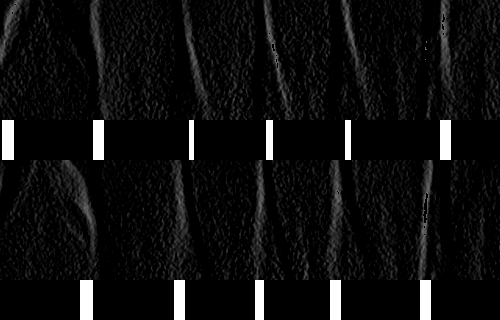
\includegraphics[height=60mm]{teeth_horizontal_1.png}
 \caption{The top image shows the left edges from the horizontal strip of the bottom teeth with the thresholded averages of the columns below it. The bottom image shows the right edges.}
\end{figure}
\bibliography{bib} 
\bibliographystyle{ieeetr}

\begin{figure}[]
\centering
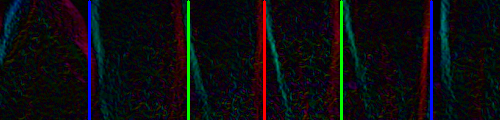
\includegraphics[height=25mm]{teeth_horizontal_2.png}
 \caption{The bottom teeth segmented by X coordinate.}
\end{figure}

\subsection{Individual teeth Y coordinates}
Once the borders between the teeth are found, we can construct a vertical line that goes through the middle of each tooth. Just like with the first step the Y coordinate can be calculated by taking a narrow vertical strip, calculating the average for each row and thresholding the result. The X coordinate from the vertical line combined with the Y coordinate found in this step will be the starting point for the fitting algorithm for this specific tooth.

\begin{figure}[]
\centering
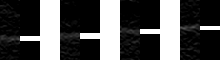
\includegraphics[height=25mm]{teeth_vertical_individual.png}
 \caption{Narrow vertical strips along the center line of each of the four bottom teeth. The horizontal white line in the bar on the right shows where the edge of the tooth is.}
\end{figure}
\bibliography{bib} 
\bibliographystyle{ieeetr}

\begin{figure}[]
\centering
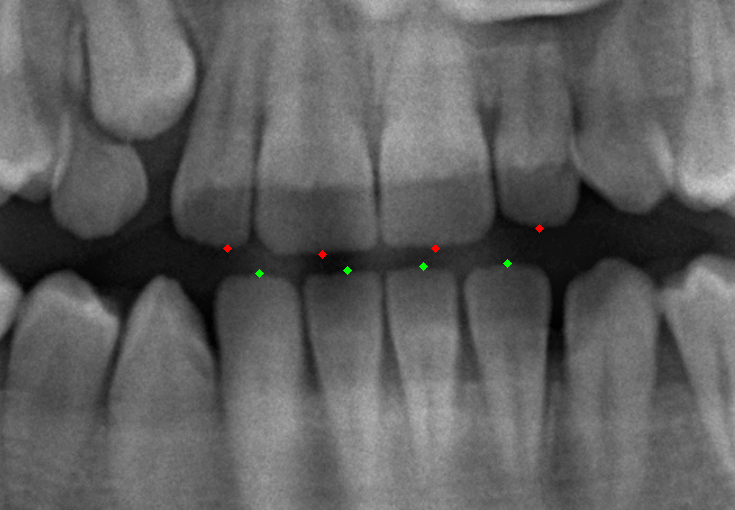
\includegraphics[height=70mm]{starting_positions.png}
 \caption{The final result of the algorithm described in the section. It shows that each starting position is roughly in the center of the upper/lower edge for the lower/upper teeth respectively.}
\end{figure}

\newpage
\section{Fitting the model}
With the Active Shape Models calculated, the radiographs processed and the starting positions determined, the fitting algorithm has everything that it needs to function. The starting positions are still not perfect and they do not account for different orientations or different shapes for the teeth. Because the shape fitting algorithm searches locally, all these factors need to be taken into account from the start to make sure that the fitting algorithm starts relatively close to the correct result. Specifically: 3 different orientations combined with 3 different shapes (3 standard deviations in each direction for the first coordinate in feature space) combined 5 different X positions around the starting point are checked. This is a total of 45 individual models per tooth as starting positions.
\\\\
From these starting positions, a deformable contour snaking algorithm is used to fit it to the actual shape of each tooth. For each landmark in the model, the costs in its neighborhood are calculated. This is calculated based on 3 factors: elasticity cost, curvature cost and external cost. The elasticity cost pushes the points towards a pattern where consecutive points are at the same distance from eachother. This prevents the points from clumping up. The curvature cost is determined by how sharp the curves are when going from point to point. The teeth are relatively smooth and round shapes, so irregular and pointy shapes should be punished. The external cost is the only cost that is actually based on the image. It is based on gradient vectors and intensity of the Sobel image. Because the points are sorted in a counter-clockwise pattern, they should only follow left edges when going down, bottom edges when going right, right edges when going up and top edges when going left. This is done by calculating the vector from the previous point to every possible position in the neighborhood of the current point. After that, the perpendicular vector to this vector is calculated and the scalar product between this vector and the gradient vector on the same position will determine the external cost for that specific position.
\\\\
These 3 cost maps are combined in a weighted sum and for each point is moved to the cheapest position in its neighborhood. This, however, does not take the actual shape of the model in account other than the very basic curvature cost. To take the shape of the tooth into account, the model is projected into the feature space for that tooth. Once its coordinates are known, any coordinate more than 3 standard deviations away is reset to the maximum of 3 standard deviations. Coordinates below 3 standard deviations are left as-is. These standard deviations are calculated based on the training data used to construct the Active Shape Models. Once all coordinates are within reasonable bounds, the model is reconstructed in 2D space.
\\\\
This reconstructed model has a good shape, but ignores the image again. This is an issue, especially in early iterations when the points have not had a chance to settle around the edge of a tooth. To fix that, the reconstructed model and the cost-optimal model are combined in a weighted average. In early iterations, the cost-optimal model dominates the average (80\%) while after a few iterations the reconstructed model starts taking over and eventually nearly entirely (90\%) determines the final shape. In total, 8 iterations are executed.
\\
To pick the best model out of the 45 models after the 8 iterations, the costs of the models are compared. The model with the lowest cost is picked.
\begin{figure}[!h]
\begin{tabular}{cc}
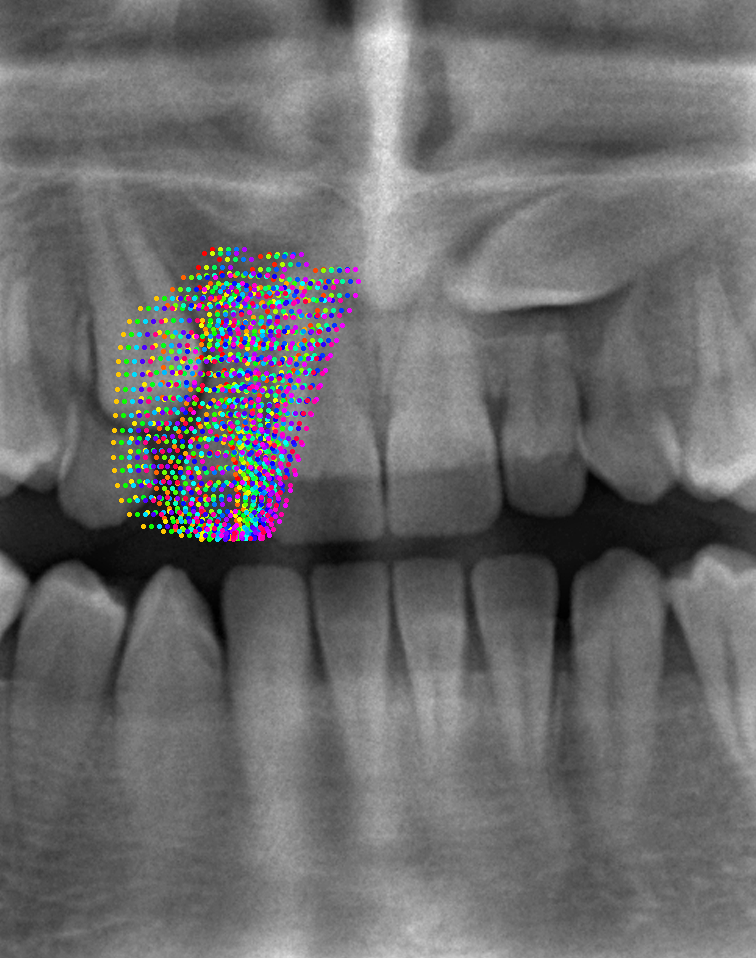
\includegraphics[width=80mm]{tooth_variations.png} & 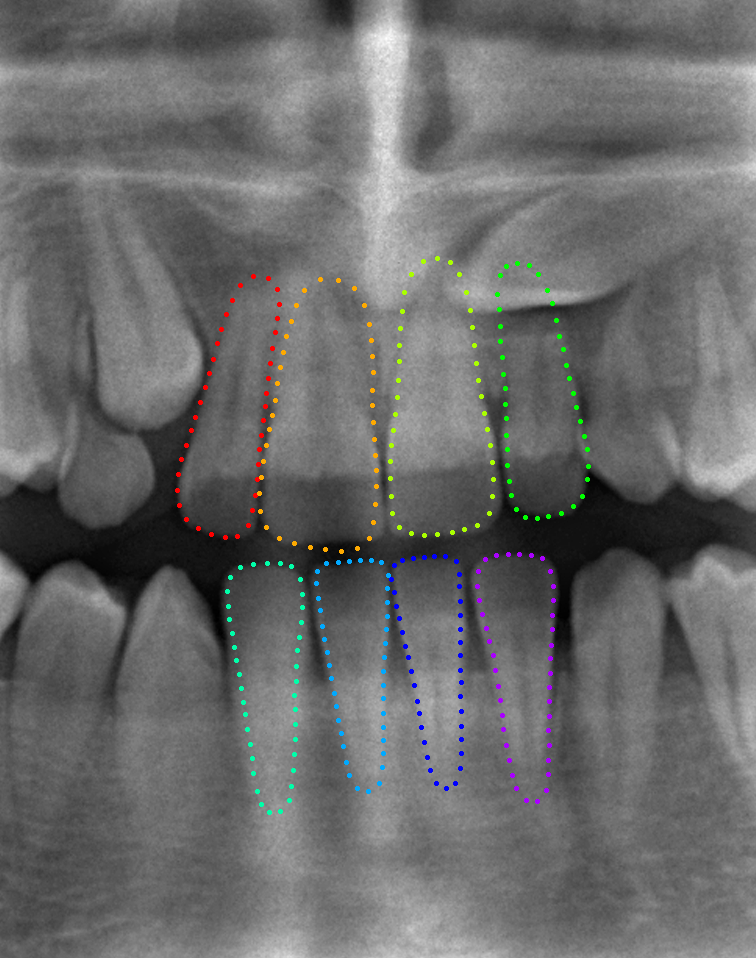
\includegraphics[width=80mm]{tooth_result_1.png}\\
 
\end{tabular}
 \caption{The left image displays all 45 initial variations for the top left tooth. The right image shows the final result of the algorithm.}
\end{figure}


\section{Weaknesses}
The algorithm in its current state has several weaknesses.

\paragraph{Metal objects} In some of the radiographs, metal objects are visible. These are mostly braces, but also includes the support for prosthetic teeth, etc. Some effort has been made to deal with these cases, but the algorithm is far from robust in these cases. More advanced processing on the radiographs needs to be done specifically to detect and remove these metal objects from the image before the rest of the algorithm runs. As it stands now, these high contrast features are misleading the algorithm in both when determining the starting positions and when actually fitting the models.

\begin{figure}[!h]
\begin{tabular}{ccc}
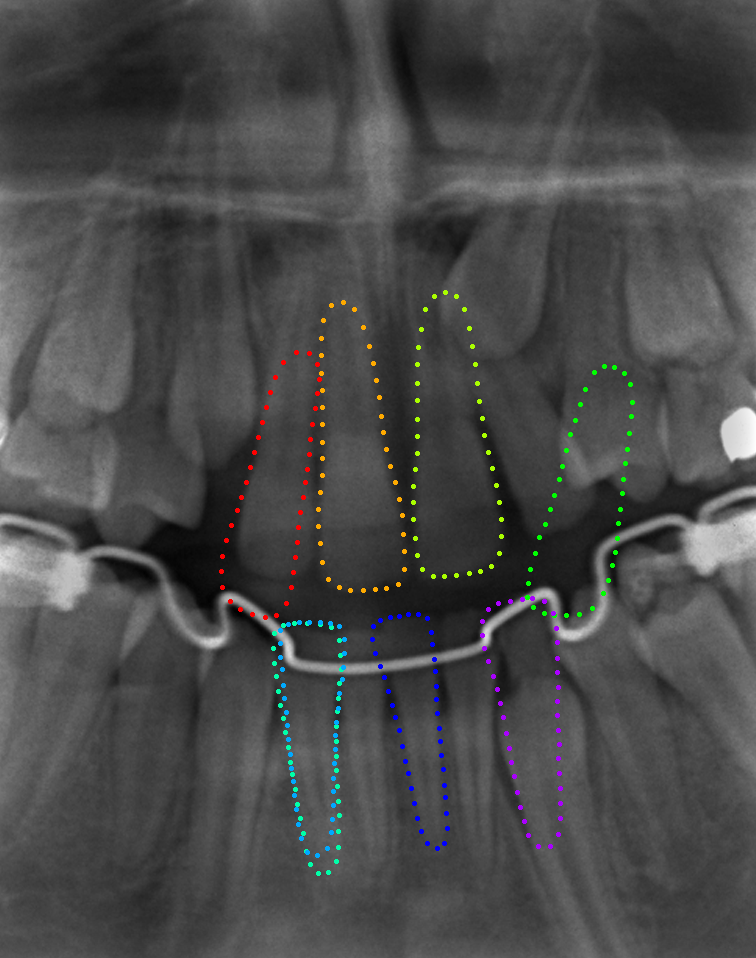
\includegraphics[width=50mm]{tooth_result_9.png} & 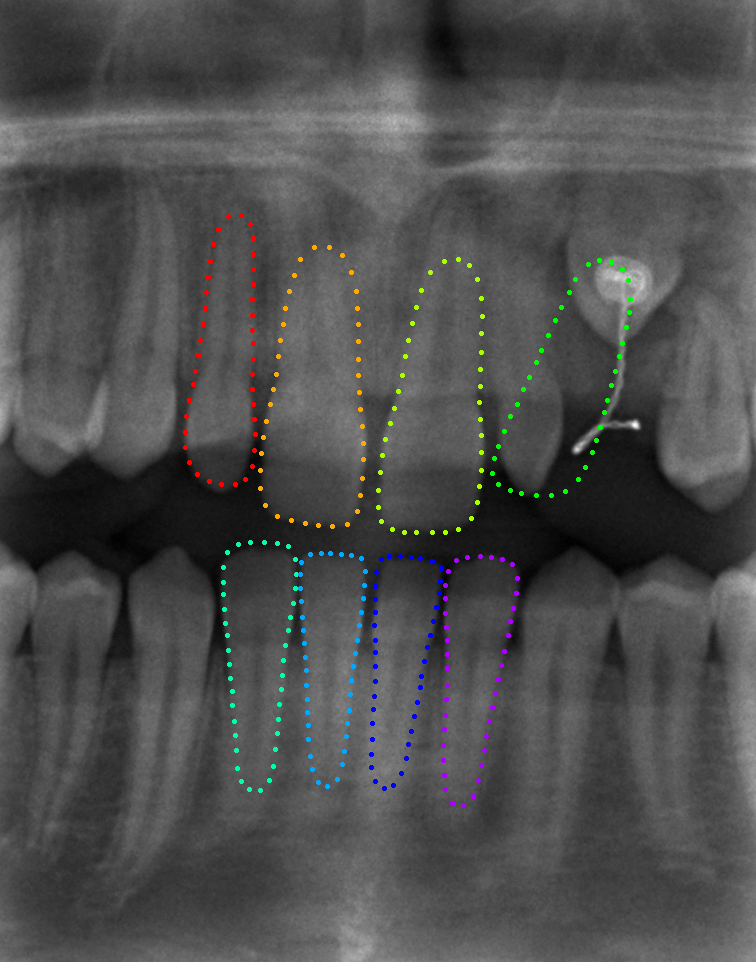
\includegraphics[width=50mm]{tooth_result_2.png} & 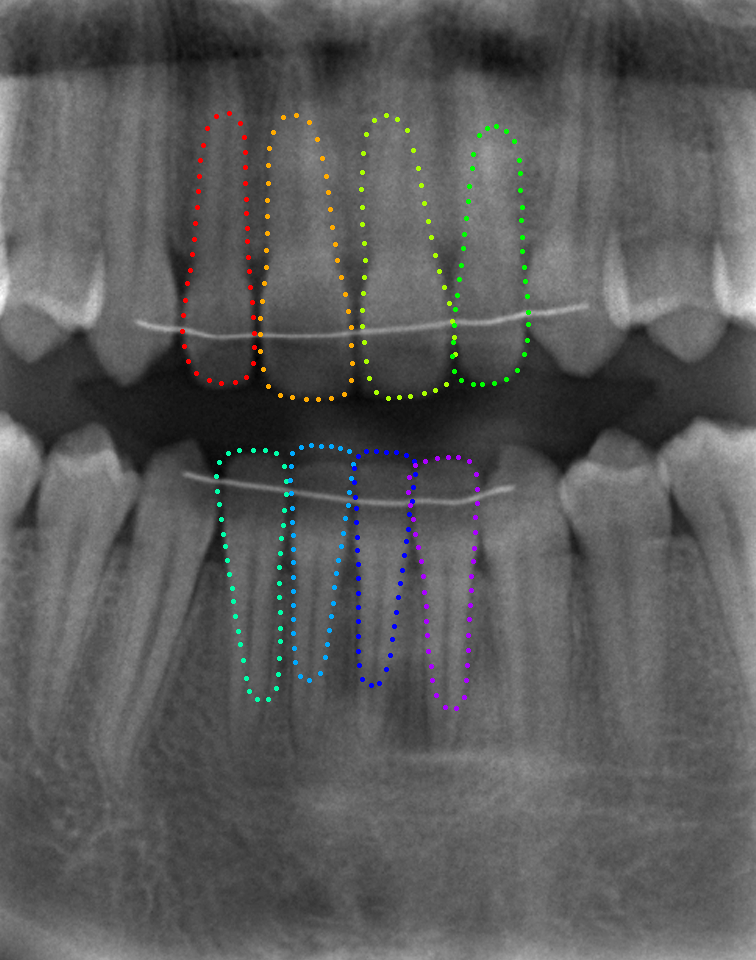
\includegraphics[width=50mm]{tooth_result_10.png} \\
 
\end{tabular}
 \caption{The left image shows a case where the metal objects have caused the starting positions of the 2 other top teeth to be much too low. The middle image shows a case where the starting position was correct, but the metal object has caused the fitting algorithm to follow the high contrast edge. The right image shows a case where the algorithm did end producing a good result even though there are metal objects in the radiograph.}
\end{figure}

\paragraph{Noise and contrast} The algorithm that determines the starting positions heavily relies on both low noise and high contrast features. However, these two qualities are at odds with eachother. Increasing contrast usually also increases the noise, while reducing noise also tends to reduce the contrast. The current processing steps do an okay job at optimizing both qualities, but I am convinced that there is a lot of room for improvement. The starting position algorithm has some instances where different sensitivies are used for the thresholds based on the contrast of the strip that's being analyzed. It also has some basic detection of ``skipped'' edges and will fill in the gap when a tooth is detected to be about double as wide as the other teeth. However, this is far from perfect. In many cases things simply go wrong due to various reasons and the X coordinates for the teeth are off by much more than the algorithm can handle.
\\
Another important weakness is determining the initial Y coordinates of the teeth. In some radiograph, there are blobs and smudges in the mouth. This can result in incorrect Y coordinates when these smudges are detected as the top/bottom edge of the tooth. It should be possible to detect and remove these blobs from the image.

\paragraph{``Scatter shot''} Using 45 different models to detect a tooth makes it much more likely that the correct solution is found, but it also greatly increases the odds that some other shape is detected instead. In its current shape, the different teeth do not know about the other teeth. This means that in some cases the teeth will overlap or be at unrealistic positions compared to the other teeth. Building a second layer of Active Shape Models based on the positions of the teeth relative to eachother could put reasonable bound on these cases. However, I did not have time to investigate this. Another weakness of using so many models is the performance impact. 45 models for each tooth means 360 models in total. That means that in total 2880 iterations have to be calculated. This limits the processing time in each iteration to a few miliseconds at most. Fewer models but a more sophisticated fitting algorithm could yield better results in less time.

\paragraph{Irregular mouths} The algorithm that determines the initial starting positions works fairly well (with the caveats given above) for normal teeth, but quickly fails when the teeth and their positions are less regular. These irregular positions and shapes of teeth usually also mean that there's likely significant overlap. This breaks the assumption of the algorithm that the teeth are mostly disjunct (as this impacts the order in which edges are found). Edge cases can be solved, but this manual approach does not scale well.

\begin{figure}[!h]
\begin{tabular}{ccc}
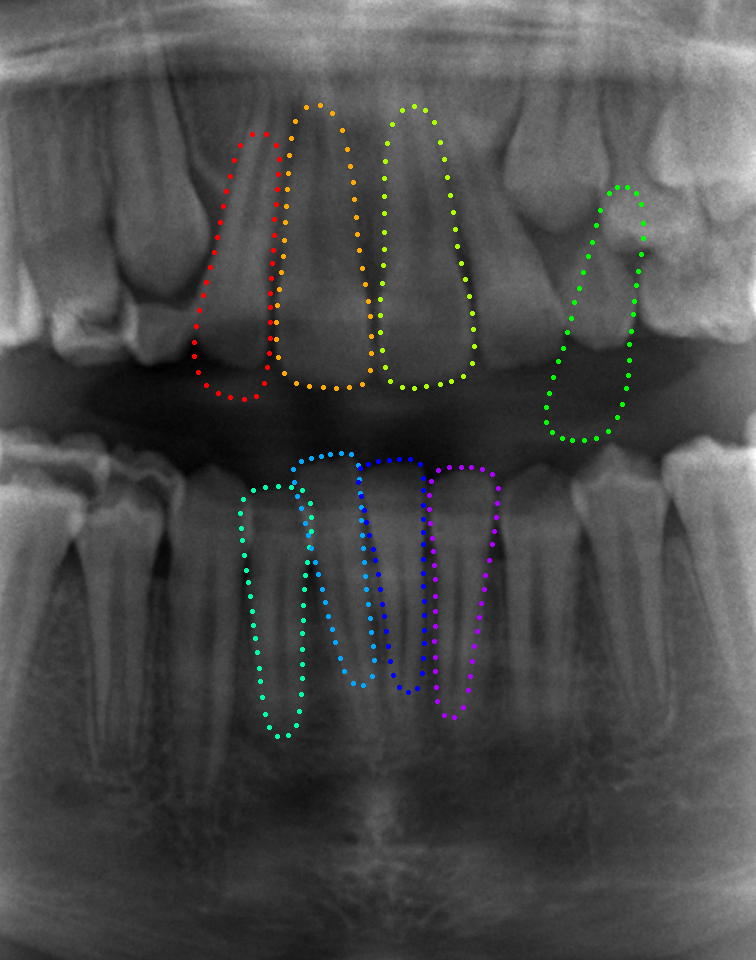
\includegraphics[width=50mm]{tooth_result_13.png} & 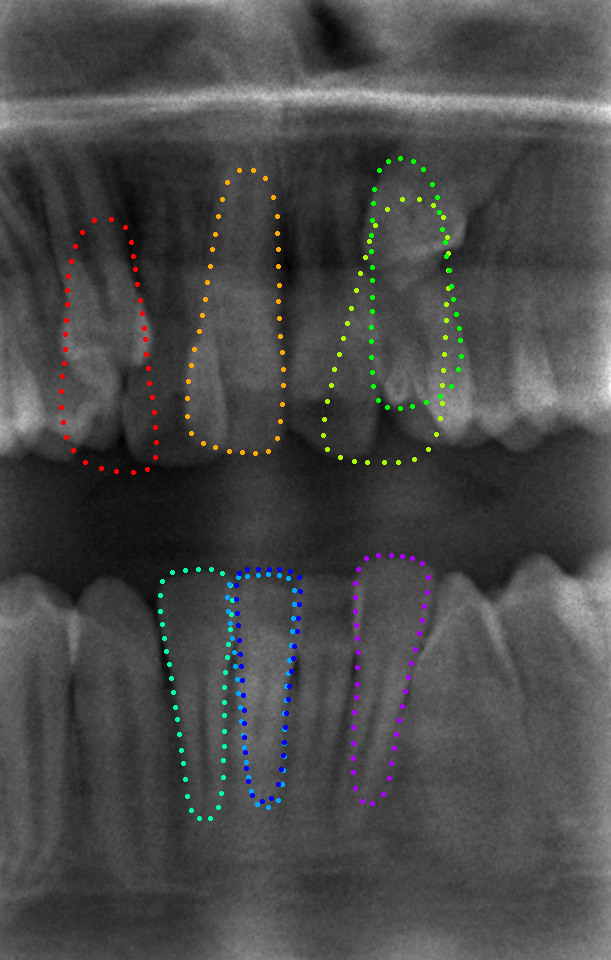
\includegraphics[width=50mm]{tooth_result_22.png} & 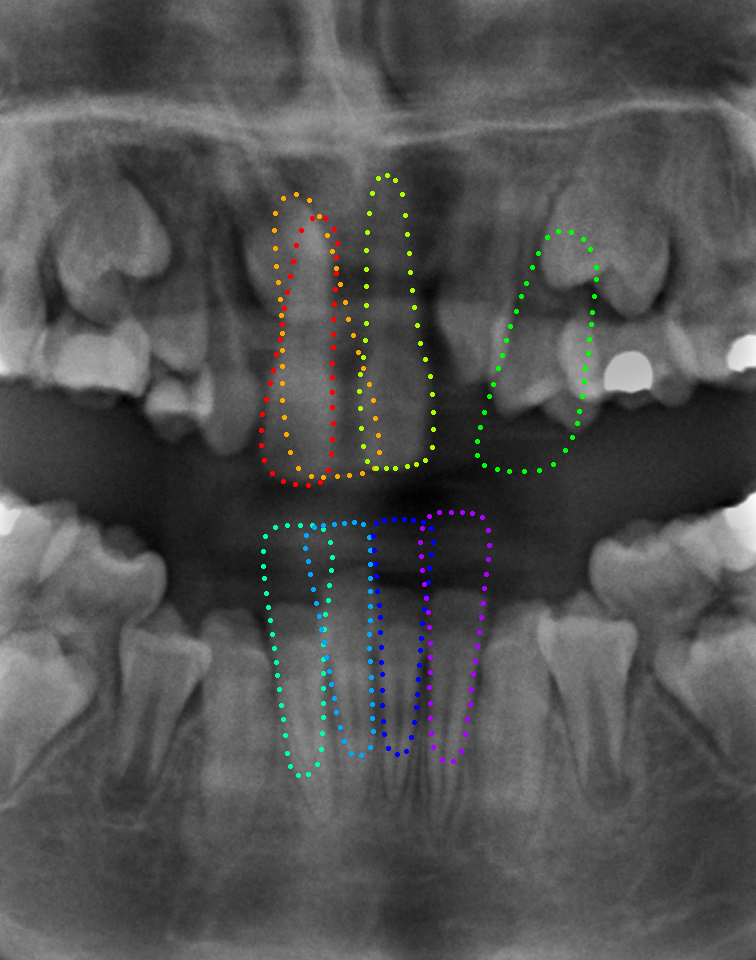
\includegraphics[width=50mm]{tooth_result_16.png}\\
 
\end{tabular}
 \caption{The left image shows the effect of blobs and smudges on the vertical initial positions of the two outer top teeth. The middle image shows 2 bottom teeth overlapping as well as some serious issue with the top teeth because of the irregular shapes. The image on the right shows more effects from smudges on the bottom row as well as the impact of irregular teeth on the top row. }
\end{figure}

\section{Tests}
To test the algorithm, I have decided to build the Active Shape Models with one of each of the 14 complete datasets left out. This model is then used to test the accuracy of the model for that specific dataset. To measure the accuracy, the percentage of overlap between the ground truth model and the result of my algorithm. This percentage is calculated by dividing the area where the models overlap by the total area of the two models combined.

\begin{figure}[!h]
\centering
\begin{tabular}{r|l}
image number & Overlap ( \%) \\
\hline
1 & 80.7	\\
2 & 71.7	\\
3 & 74.1	\\
4 & 74.2	\\
5 & 26.3	\\
6 & 86.5	\\
7 & 76.5	\\
8 & 76.5	\\
9 & 48.6	\\
10 & 43.5	\\
11 & 81.0	\\
12 & 69.7	\\
13 & 63.3	\\
14 & 77.3	\\
\hline
average & 67.7
\end{tabular}
\end{figure}

\begin{figure}
\captionsetup[subfigure]{labelformat=empty}
\begin{subfigure}{.33\textwidth}
\centering
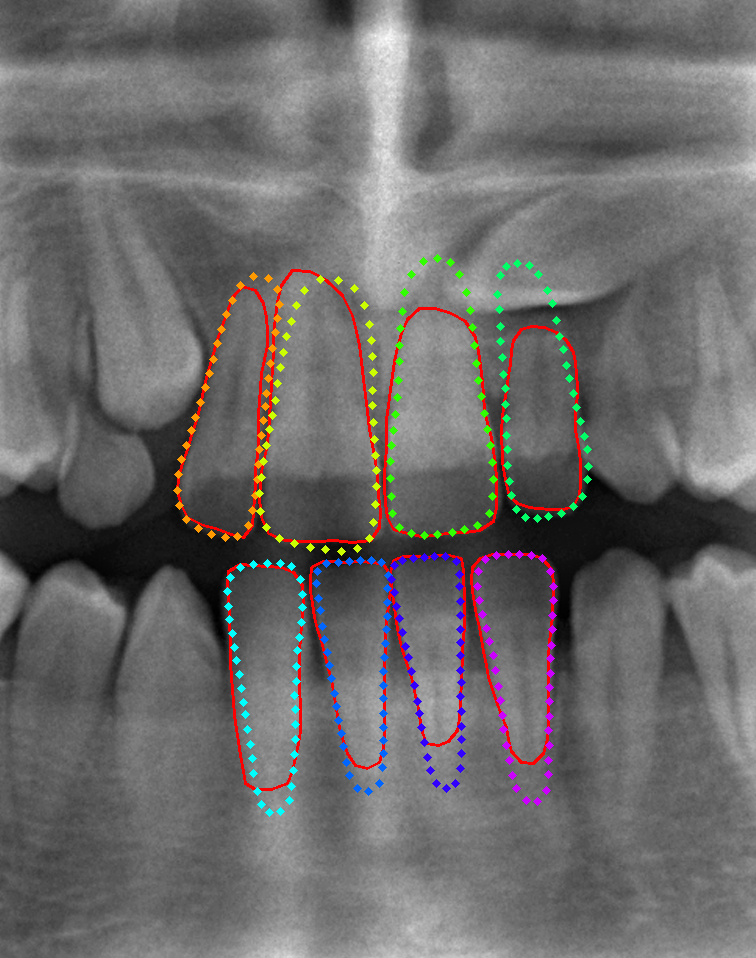
\includegraphics[width=50mm]{tooth_result_overlay_1.png}
\caption{Radiograph 1: 80.7\%}
\end{subfigure}%
\begin{subfigure}{.33\textwidth}
\centering
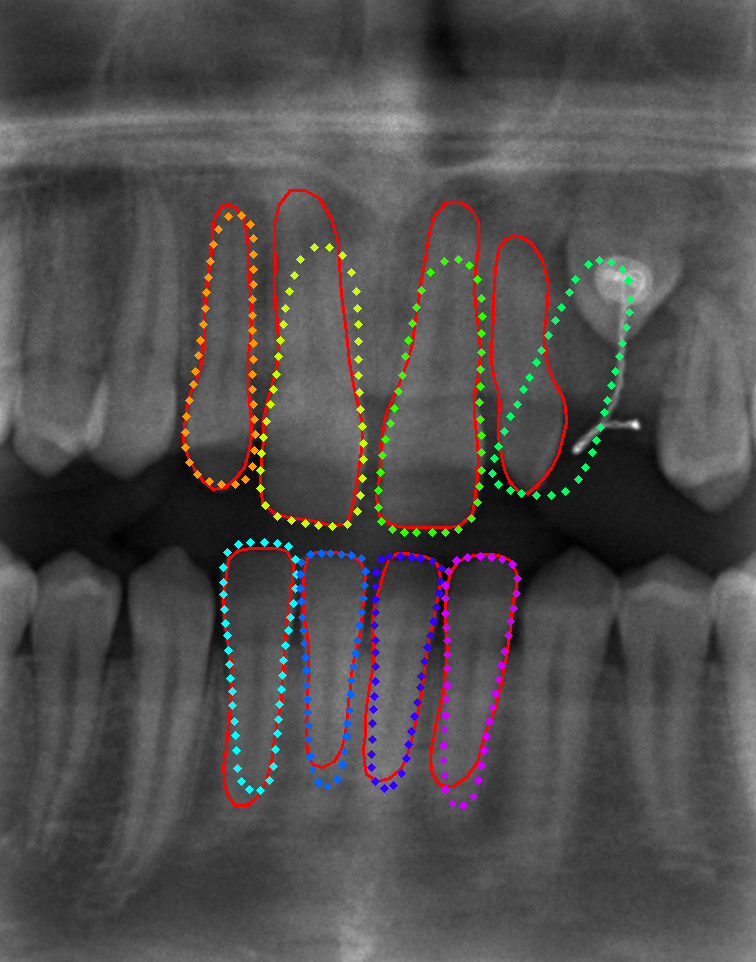
\includegraphics[width=50mm]{tooth_result_overlay_2.png}
\caption{Radiograph 2: 71.7\%}
\end{subfigure}%
\begin{subfigure}{.33\textwidth}
\centering
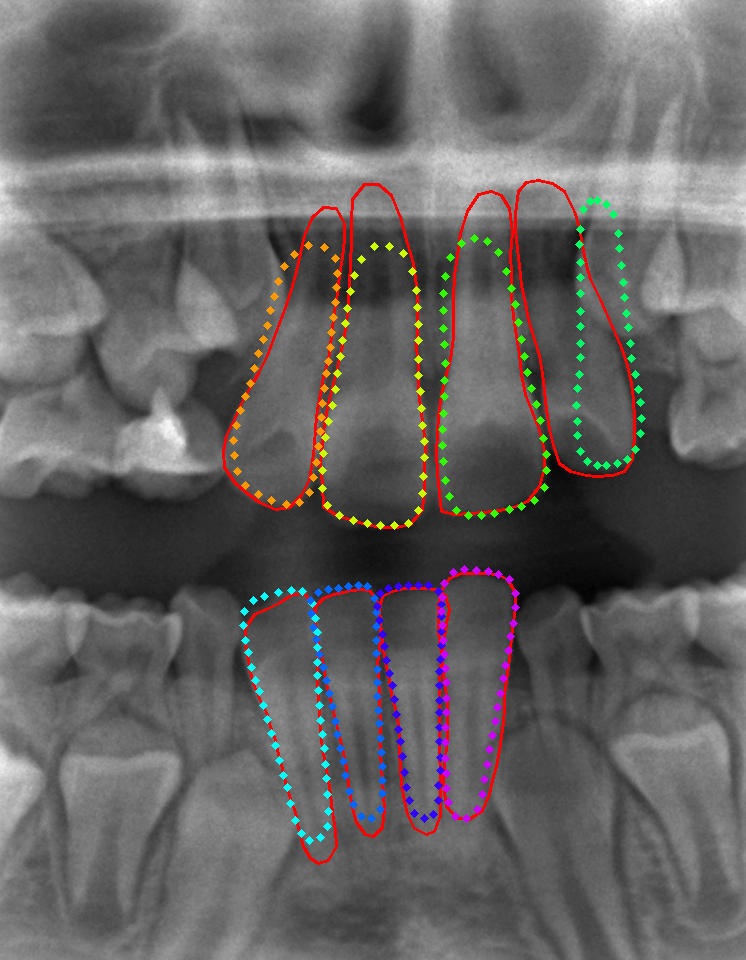
\includegraphics[width=50mm]{tooth_result_overlay_3.png}
\caption{Radiograph 3: 74.1\%}
\end{subfigure}%

\begin{subfigure}{.33\textwidth}
\centering
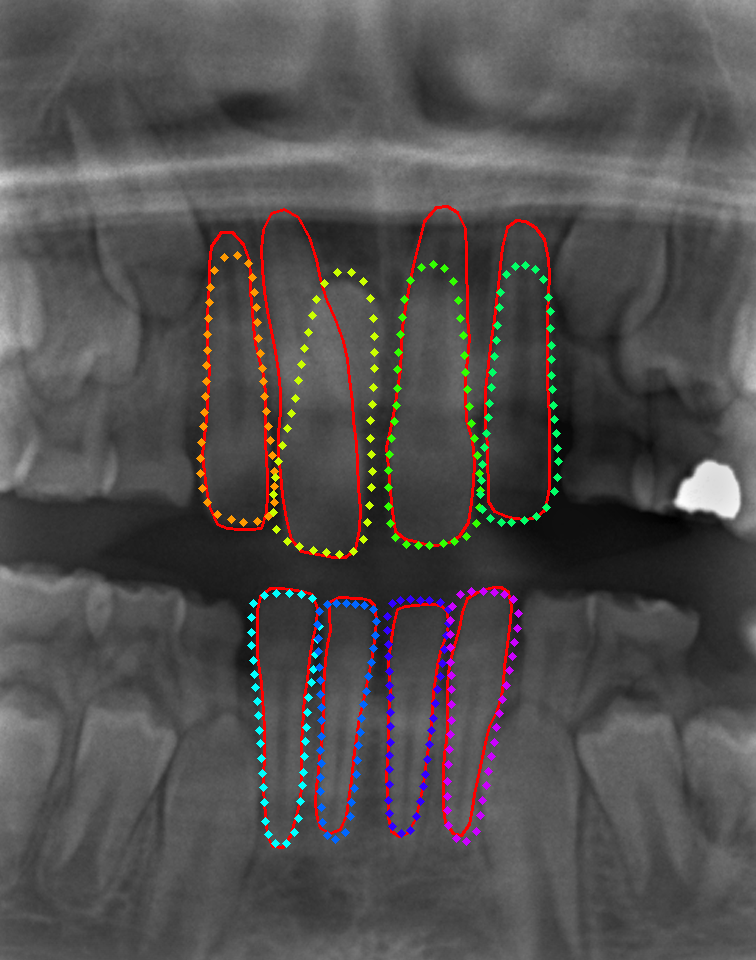
\includegraphics[width=50mm]{tooth_result_overlay_4.png}
\caption{Radiograph 4: 74.2\%}
\end{subfigure}%
\begin{subfigure}{.33\textwidth}
\centering
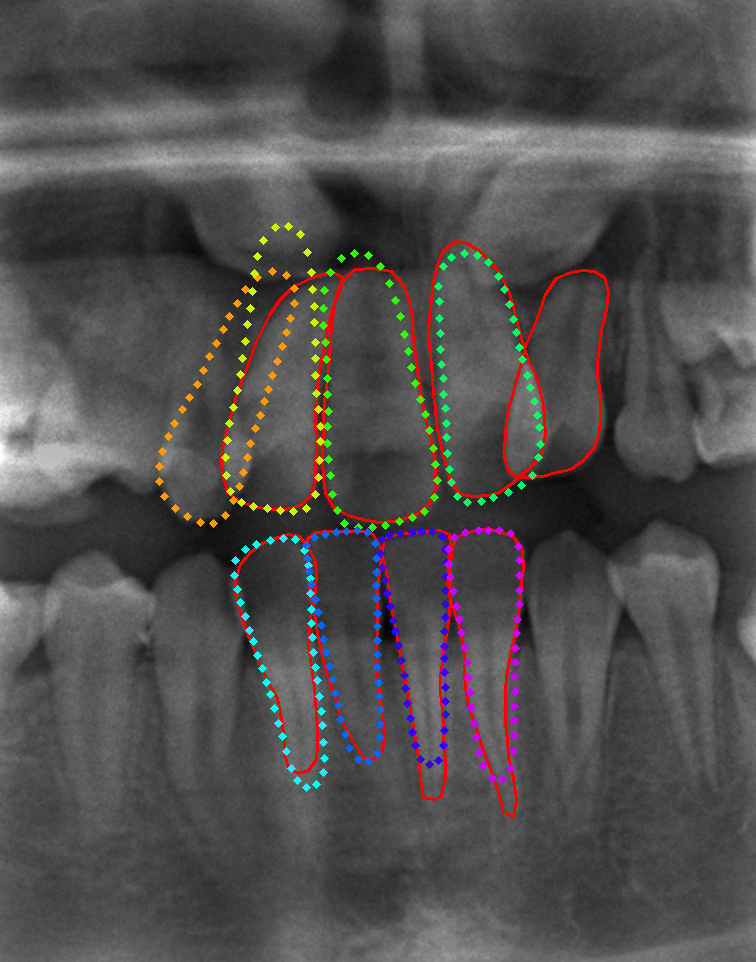
\includegraphics[width=50mm]{tooth_result_overlay_5.png}
\caption{Radiograph 5: 26.3\%}
\end{subfigure}%
\begin{subfigure}{.33\textwidth}
\centering
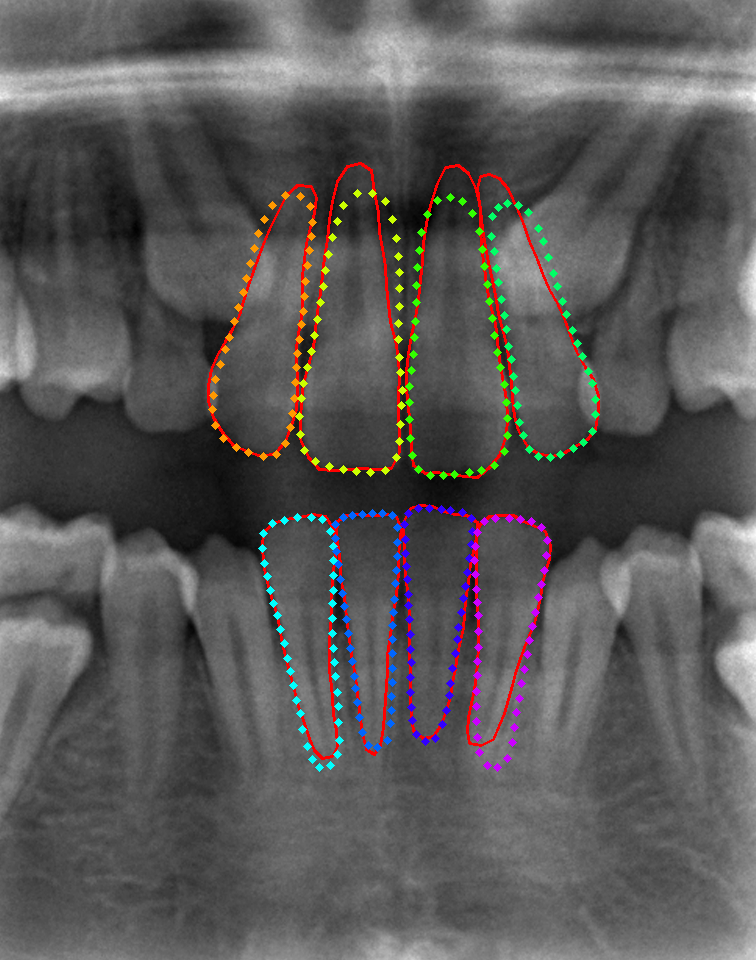
\includegraphics[width=50mm]{tooth_result_overlay_6.png}
\caption{Radiograph 6: 86.5\%}
\end{subfigure}%

\begin{subfigure}{.33\textwidth}
\centering
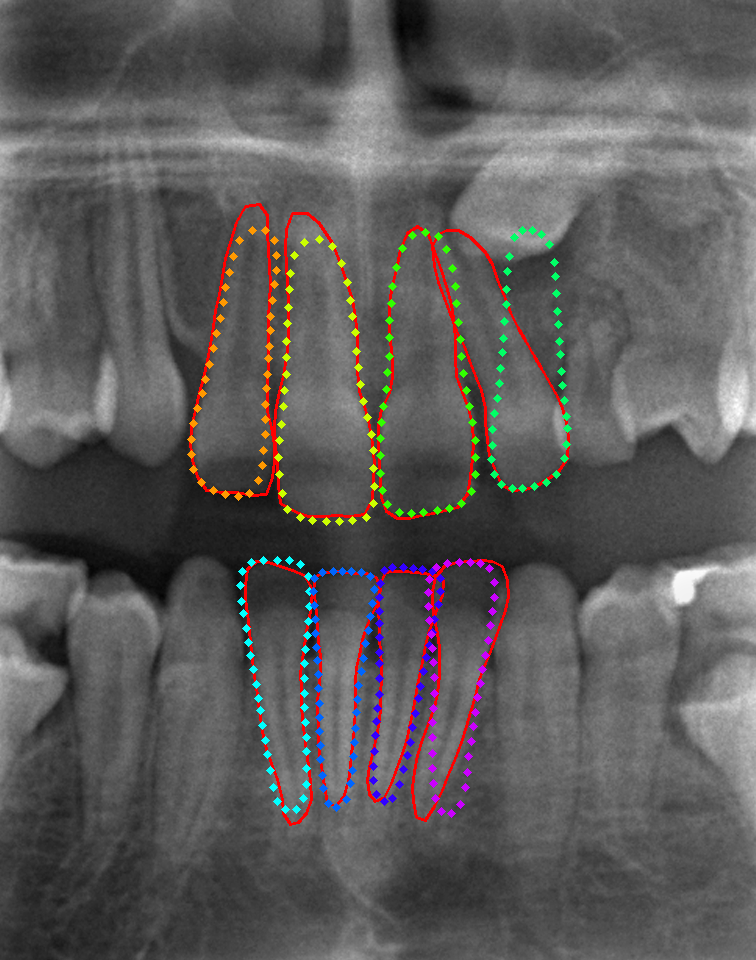
\includegraphics[width=50mm]{tooth_result_overlay_7.png}
\caption{Radiograph 7: 76.5\%}
\end{subfigure}%
\begin{subfigure}{.33\textwidth}
\centering
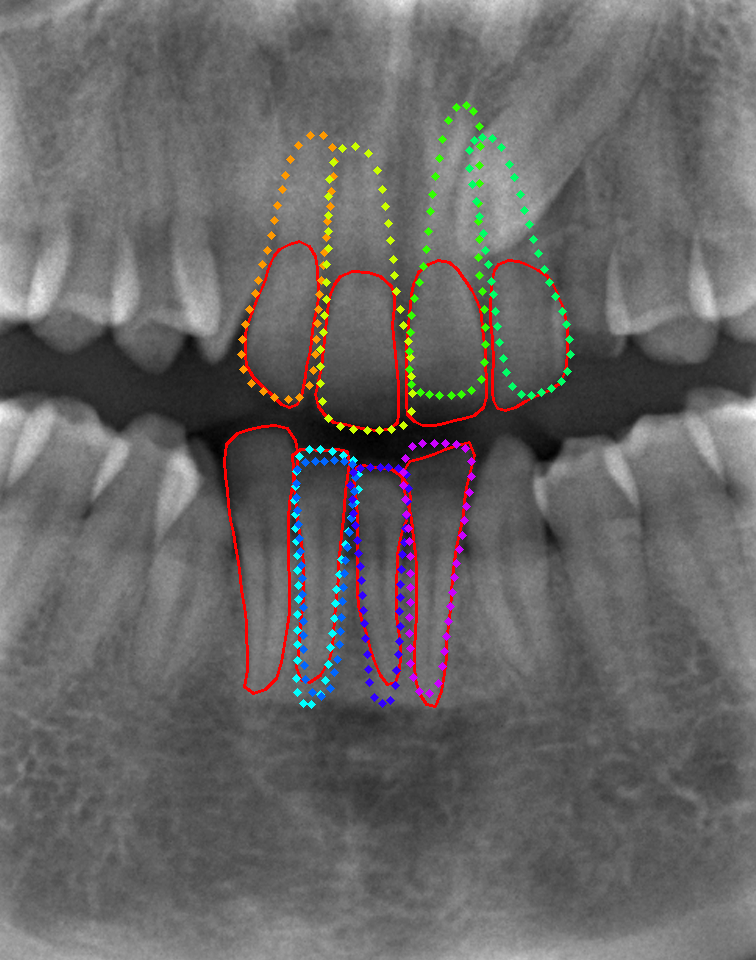
\includegraphics[width=50mm]{tooth_result_overlay_8.png}
\caption{Radiograph 8: 48.6\%}
\end{subfigure}%
\begin{subfigure}{.33\textwidth}
\centering
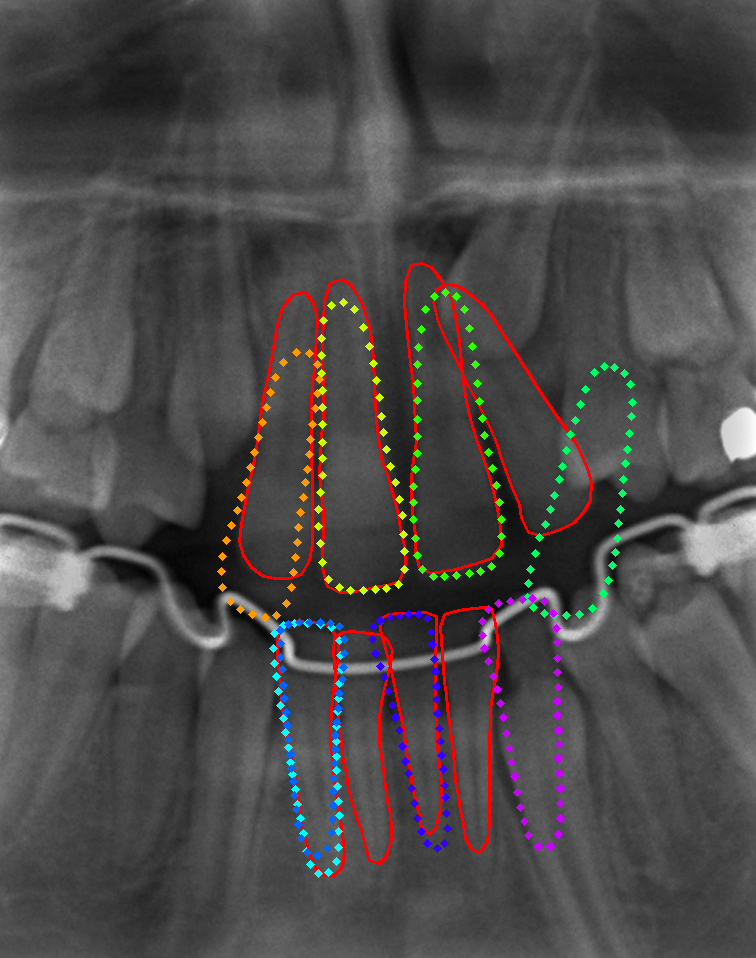
\includegraphics[width=50mm]{tooth_result_overlay_9.png}
\caption{Radiograph 9: 43.5\%}
\end{subfigure}%

\end{figure}

\begin{figure}
\captionsetup[subfigure]{labelformat=empty}
 \begin{subfigure}{.33\textwidth}
\centering
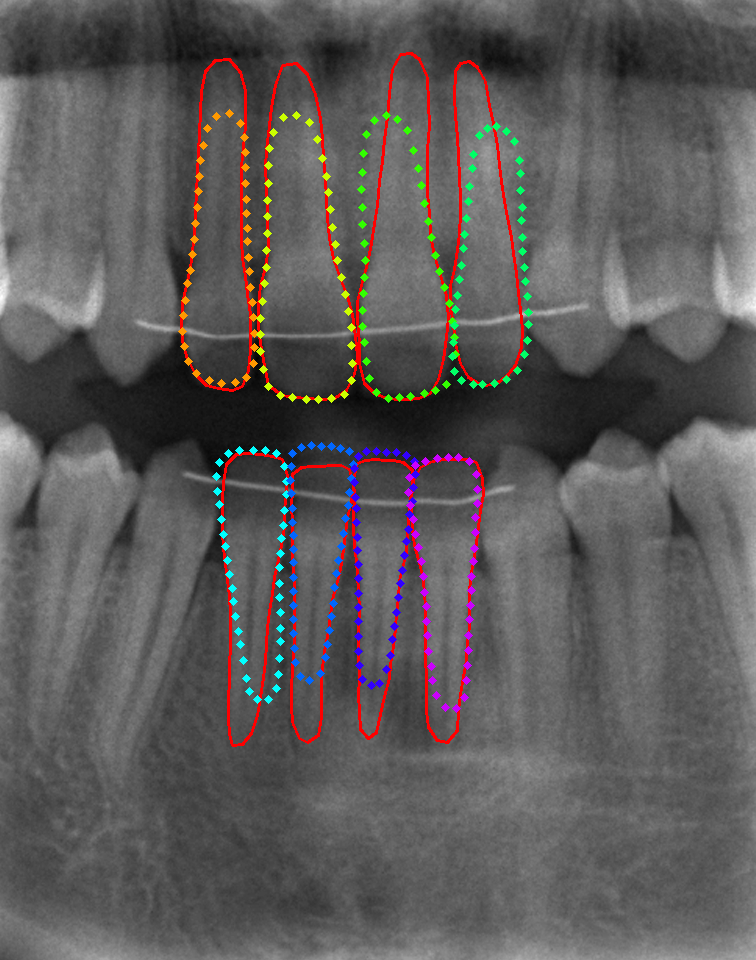
\includegraphics[width=50mm]{tooth_result_overlay_10.png}
\caption{Radiograph 10: 74.8\%}
\end{subfigure}%
\begin{subfigure}{.33\textwidth}
\centering
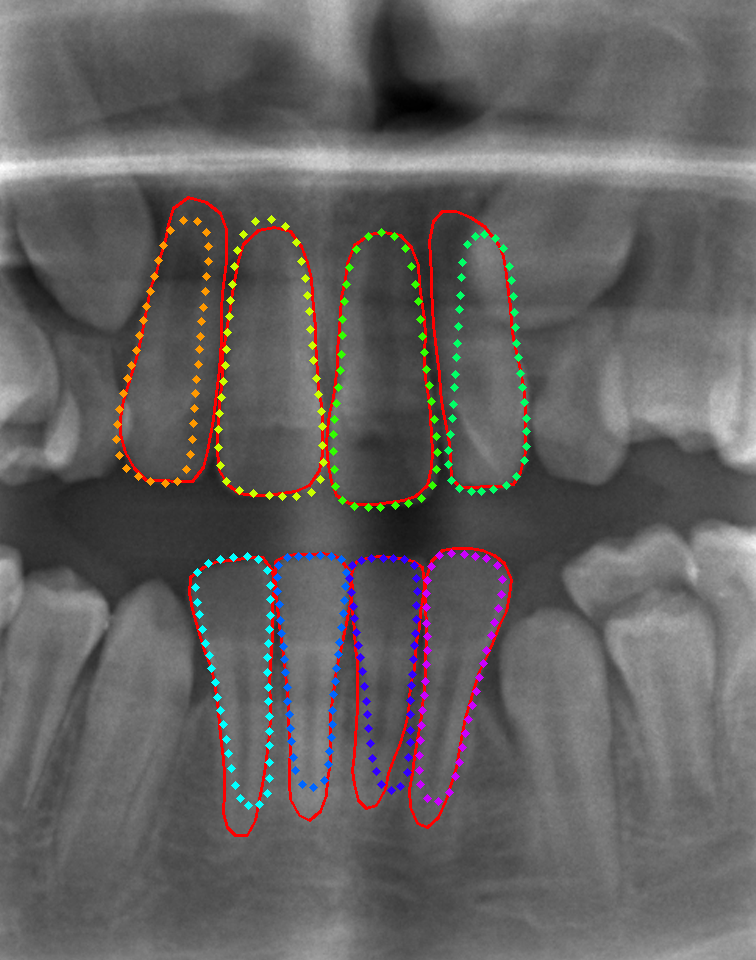
\includegraphics[width=50mm]{tooth_result_overlay_11.png}
\caption{Radiograph 11: 81.0\%}
\end{subfigure}%
\begin{subfigure}{.33\textwidth}
\centering
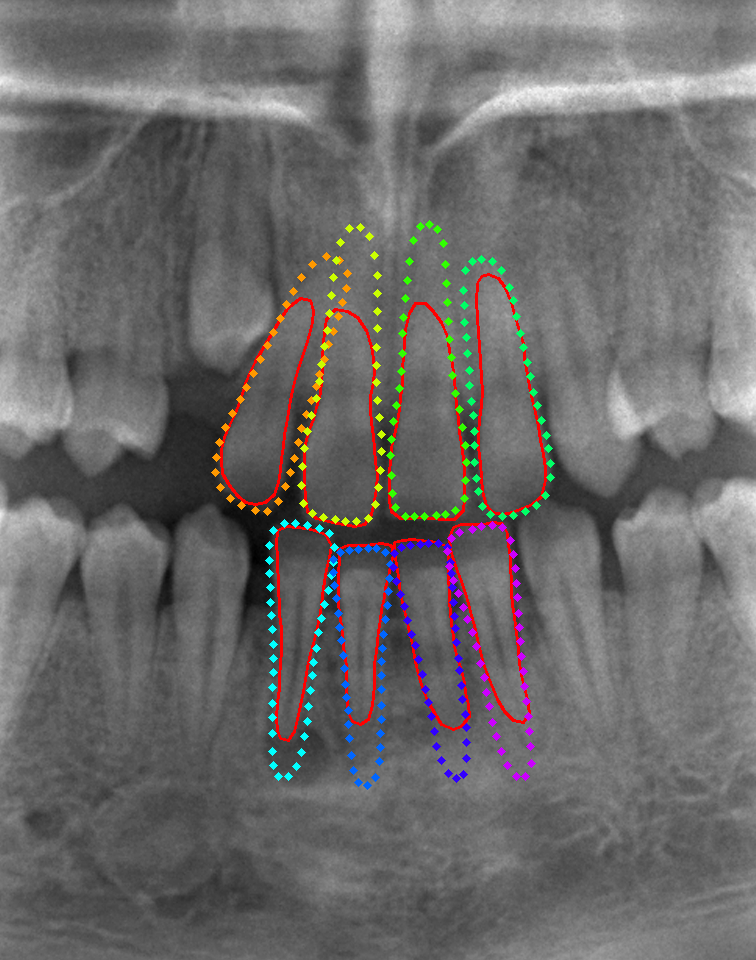
\includegraphics[width=50mm]{tooth_result_overlay_12.png}
\caption{Radiograph 12: 69.7\%}
\end{subfigure}%

\begin{subfigure}{.33\textwidth}
\centering
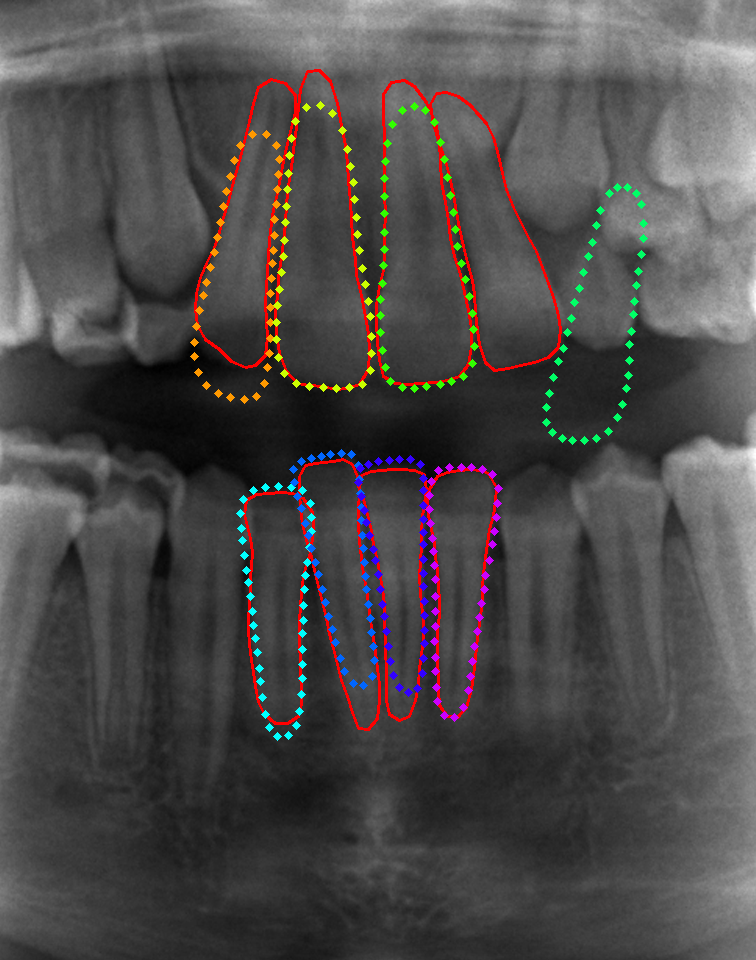
\includegraphics[width=50mm]{tooth_result_overlay_13.png}
\caption{Radiograph 13: 63.3\%}
\end{subfigure}%
\begin{subfigure}{.33\textwidth}
\centering
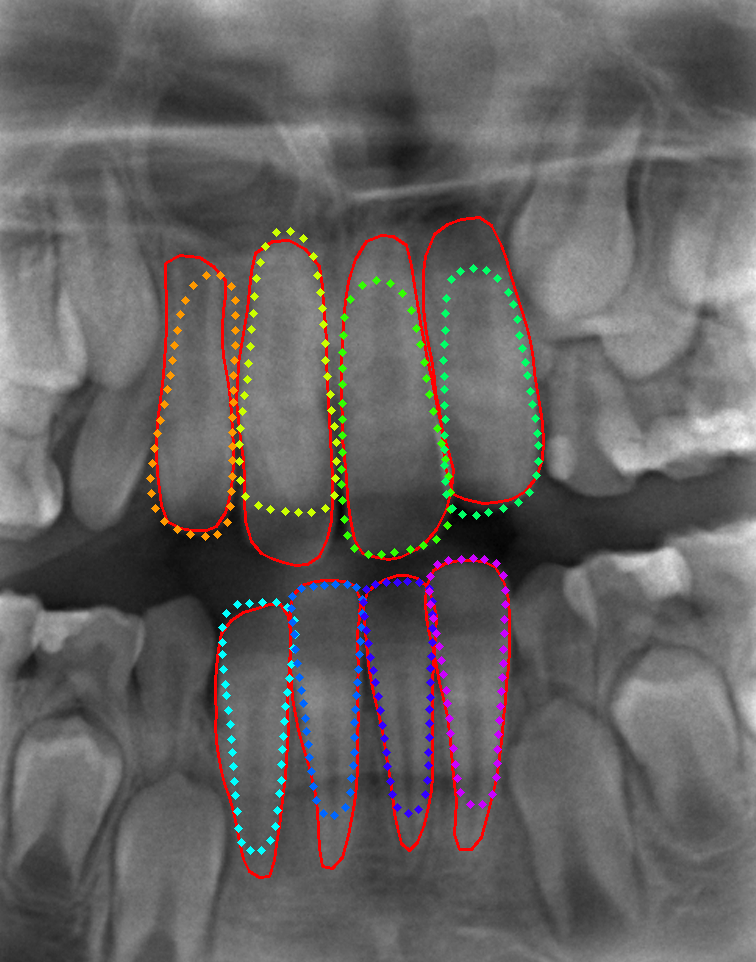
\includegraphics[width=50mm]{tooth_result_overlay_14.png}
\caption{Radiograph 14: 77.3\%}
\end{subfigure}%
\end{figure}

\section{Conclusion}
Overall, my solution provides a solid foundation but can still be improved upon in many ways. Given more time and data, there is still a lot that can be gained by improving the preprocessing, initial positions and the fitting algorithm. The algorithm to determine the initial positions was by far the hardest to get working at a reasonable level. A large amount of constants needed to be finely tuned. On a larger scale this would probably be a lot easier to do with a convolutional neural network, given a large training dataset. While the final preprocessing flow is fairly simple, I spent a lot of time trying to tease out the information I needed from the input radiographs. While the result is good enough for most radiographs right now, I am not completely satisfied with the result. There is still a lot of noise and the constrast is simply too low in certain radiographs, making the algorithm fail entirely. \\ On a whole, this has been a very interesting problem to work on. I have learned a lot from this project.
\bibliography{bib} 
\bibliographystyle{ieeetr}



\end{document}
